\section{Experiment 2: Enhancing The Training Captions}
% Corresponging Progress Reports:
% https://www.notion.so/241220-Matthias-reducing-train-data-with-care-First-AI-captions-0a0a3c610dba4d9c84d4eda4fb1c53dd
% https://www.notion.so/250110-Matthias-AICaptions-Evaluation-053ef06c3e6e4858808c9266cc1bffc0
% https://www.notion.so/20250119-Matthias-Filling-The-gaps-2-a8f598e120de4b6ba4b20a7d0a2a9253#18e2cfd830264119bbfcd90d223b4cc0

\subsection{Background}

Ich muss auf jeden Fall die Hypothese aufstellen, dass sich die Rekonstruktionsleistung von Artificial Shapes erhöht wenn ein Augenmerk auf low-level Features in den captions drin ist und für natürliche Testbilder, wenn ein Augnemerkt auf den high-level Featuers in den captions drin ist. 

\subsection{Methods}
To further investigate the performance of the Brain Diffuser algorithm, the influence of the subtitles and the cliptext translator is first tested. Possible differences that may result from the high-level vs.\ low-level information of an image are to be analysed. For this reason, additional captions are created below for the training data, focusing on either the high-level or the low-level features of the image. The API of ChatGPT\cite{OpenAI_ChatGPT_2024} was used to generate the additional captions for the training images. With this, captions with two different prompts were generated for all 1200 training images. As it was empirically found that the cliptext features can encode less information with increasing number of tokens (= caption length)\cite{zhangLongCLIPUnlockingLongText2024}, care was taken to ensure that the length of the generated captions did not exceed 35 tokens as far as possible. The two prompts used to generate the subtitles are as follows
\begin{itemize}
    \item \textbf{high-level}: Describe the visual contents of this picture. Focus on the semantic concepts in the image. What are the main subjects of the image and what is happening in it? Make sure the output doesn't exceed 25 tokens.
    \item \textbf{low-level}: Describe the visual contents of this picture without using the word representing its direct category or semantic meaning as much as possible. Instead, focus on the colors, shapes, and textures with their relative positions in the image. Do not interpret the scene just describe what is actually visible. Make sure the output doesn't exceed 25 tokens.
\end{itemize}

The number of desired tokens per generated caption can only be specified implicitly via the prompt, without cutting off a caption in the middle. Accordingly, the number of tokens actually generated varies slightly. Captions longer than 35 tokens were excluded and the prompt was repeated until a corresponding caption shorter than 35 tokens was found. On average, 30.81 tokens (std = 2.8) were generated for the low-level captions and 22.84 (std = 3.17) for the high-level captions. The higher length of the low-level captions can be explained by the fact that semantic concepts, which can usually bundle many low-level properties (e.g. `dog' vs. `creature with four legs, fur and snout'), have to be avoided. Figure~\ref{fig:aicap_caption_samples} compares the high-level and low-level captions for two images from the training dataset with the human-generated captions. It can be seen that the low-level captions do indeed largely avoid semantic descriptions and tend to describe colours, shapes and textures. The high-level captions are comparatively similar to the human-generated captions and refer to semantic concepts (e.g.\ raccoon or can).

\begin{figure}[ht]
    \centering
    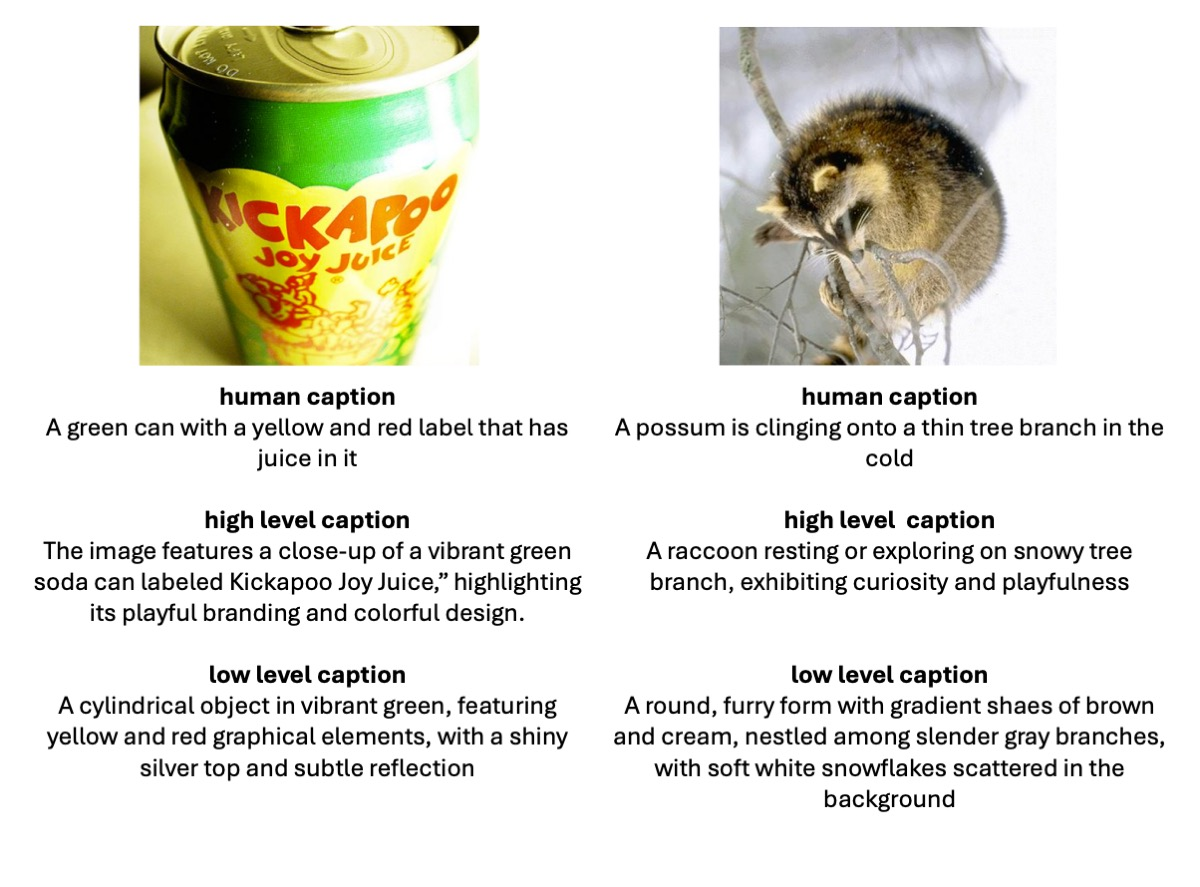
\includegraphics[width=1\textwidth]{plots/aicap_samples.jpeg}
    \caption{Captions with different prompts}\label{fig:aicap_caption_samples}
\end{figure}

The generated captions were subsequently used to train the Brain Diffuser's cliptext encoder. The clipvision and VDVAE components of the brain-diffuser do not change as a result, so only the performance of the cliptext translator is reported. For an extended baseline against which to compare the AI-generated subtitles, the human-generated subtitles are shuffled in an additional test condition. Thus, in this condition the captions have nothing to do with the actual image content, the translator should not be able to learn to make any meaningful predictions, just as the reconstructions produced with the translator trained with shuffled captions should be worse than with the normal baseline. In the Translator, the human-generated captions are used as test data for all comparisons to ensure comparability between conditions (i.e.\ the same test data is used for all conditions). 

When reconstructing with the Versatile Diffusion algorithm in the Brain Diffuser, the mixing parameter, which determines the influence of the cliptext features on the final reconstruction, is set to 0.4 and 0.8 respectively. In the original publication of the brain-diffuser\cite{ozcelikNaturalSceneReconstruction2023} the mixing parameter was 0.4, but in order to obtain a stronger influence of the captions and thus to be able to better evaluate the differences in the captions, the reconstructions are additionally analysed here with the parameter 0.8.


\subsection{Results}

\subsubsection{Translator Performance}

\begin{figure}[ht]
    \centering
    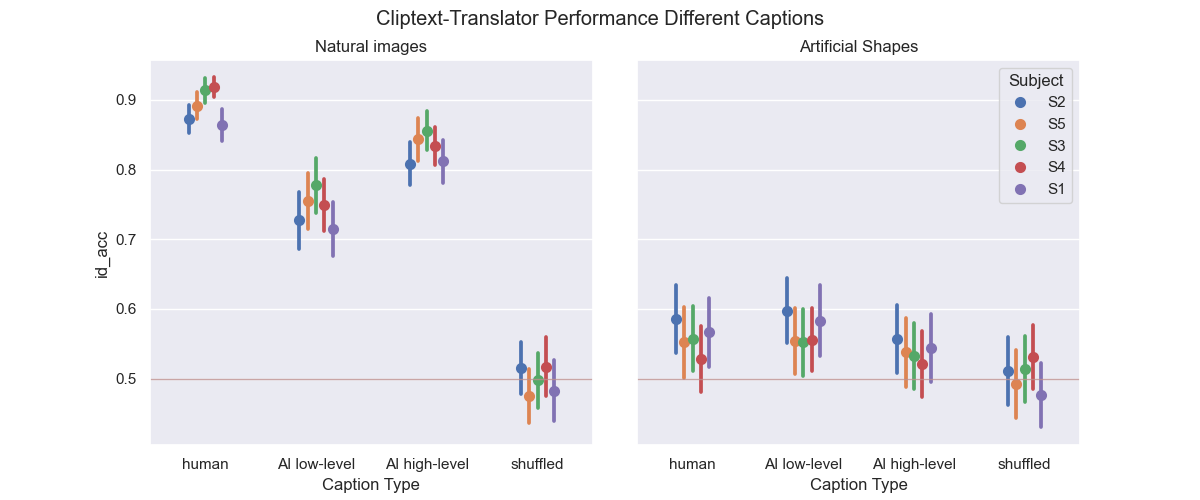
\includegraphics[width=0.9\textwidth]{plots/aicap_translator.png}
    \caption{AI-cap translator}\label{fig:aicap_translator}
\end{figure}

Figure~\ref{fig:aicap_translator} shows the results of the cliptext translator for both the natural test images and the artificial shapes. The effects can be seen very clearly for the natural test images, the identification accuracy of the translator trained with the human-generated captions is the highest. This is not surprising, as the test data for all conditions were also the human-generated captions of the test images, and therefore there is a slight domain mismatch for the AI data captions (the training data is generated by the AI, the test data by humans). The translator trained with shuffled training data is exactly at random probability, so the cliptext features could rightfully not be predicted. Both conditions with the AI-generated test data are also significantly better than random probability, with the high-level captions performing slightly better than the low-level captions (as noted above, the high-level captions also have a higher agreement with the human-generated captions). 


The results for artificial shapes are very different. Again, shuffled training data can predict results only at the random level; all other translators also show improved performance compared to the shuffled test data (and thus improved performance compared to the random level). In this condition, however, the translators trained with AI-generated high-level captions perform worse than those trained with low-level captions. The translator trained on the human-generated captions also appears to outperform the AI-generated high-level captions, although the result is somewhat less clear. 

\subsubsection{Reconstruction Performance}


The quantitative performance of the reconstructions for the natural test images is shown in Figure~\ref{fig:aicap_reconstruction_test_both_mixings} and for the artificial shapes in Figure~\ref{fig:aicap_reconstruction_art_both_mixings}. The results for mixing parameters 0.4 and 0.8 are shown for each type of caption and metric. The natural test images show that the differences between the individual captions with a mixing parameter of 0.4 are very small. Even the reconstructions with shuffled captions are only slightly worse with a mixing of 0.4 than with valid captions. The differences only become apparent when comparing the results with a mixing of 0.8. First, it can be observed that the pixel correlation increases for all captions as the mixing parameter increases. This is the case even for shuffled captions. An increased influence of the cliptext features therefore increases the pixel correlation in any case, even if it is a semantically incorrect influence as in the case of the shuffled captions. In the case of Dreamsim and Clip Accuracy, on the other hand, performance decreases as the mixing  increases, especially in the case of shuffled captions. For human-generated captions and high-level captions, performance degrades less with increasing mixing (or even remains constant) than for low-level captions. 
\begin{figure}[ht]
    \centering
    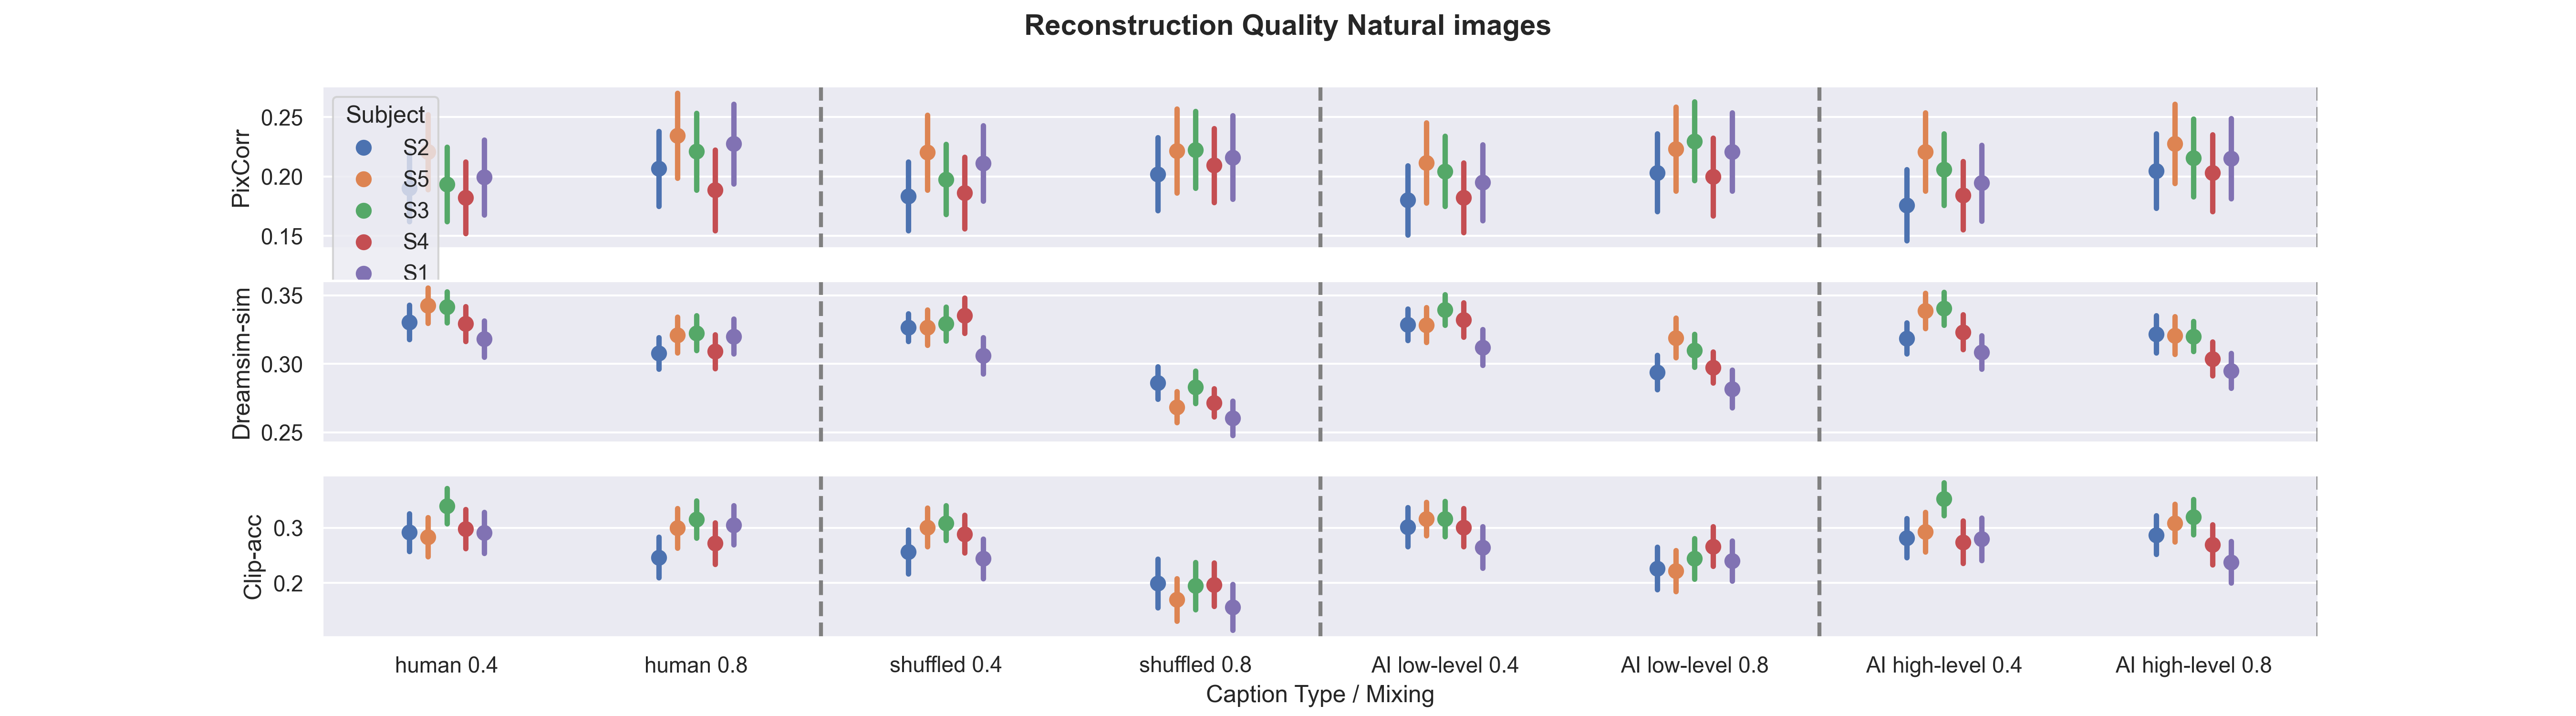
\includegraphics[width=1\textwidth]{plots/aicap_reconstruction_test_both_mixings.png}
    \caption{Reconstruction Natural Test Images with different captions}\label{fig:aicap_reconstruction_test_both_mixings}
\end{figure}


As before with the Translator, the results of the reconstruction of the artificial images are reversed. Again, with a low mixing of 0.4, there are very only few observable differences between the captions. And also as before, the pixel correlation increases with increasing mixing for all captions. But now, compared to the natural test images, the performance measured with Dreamsim Similarity also increases with increasing mixing for all captions. Especially with low level captions, good performance can be achieved with artificial images when mixing is high. The results for human and high-level captions are relatively similar and still significantly better than shuffled captions. The results for clip accuracy are very low and therefore difficult to interpret, as there is generally little semantic content in the artificial images, so the result is not surprising. 

\begin{figure}[ht]
    \centering
    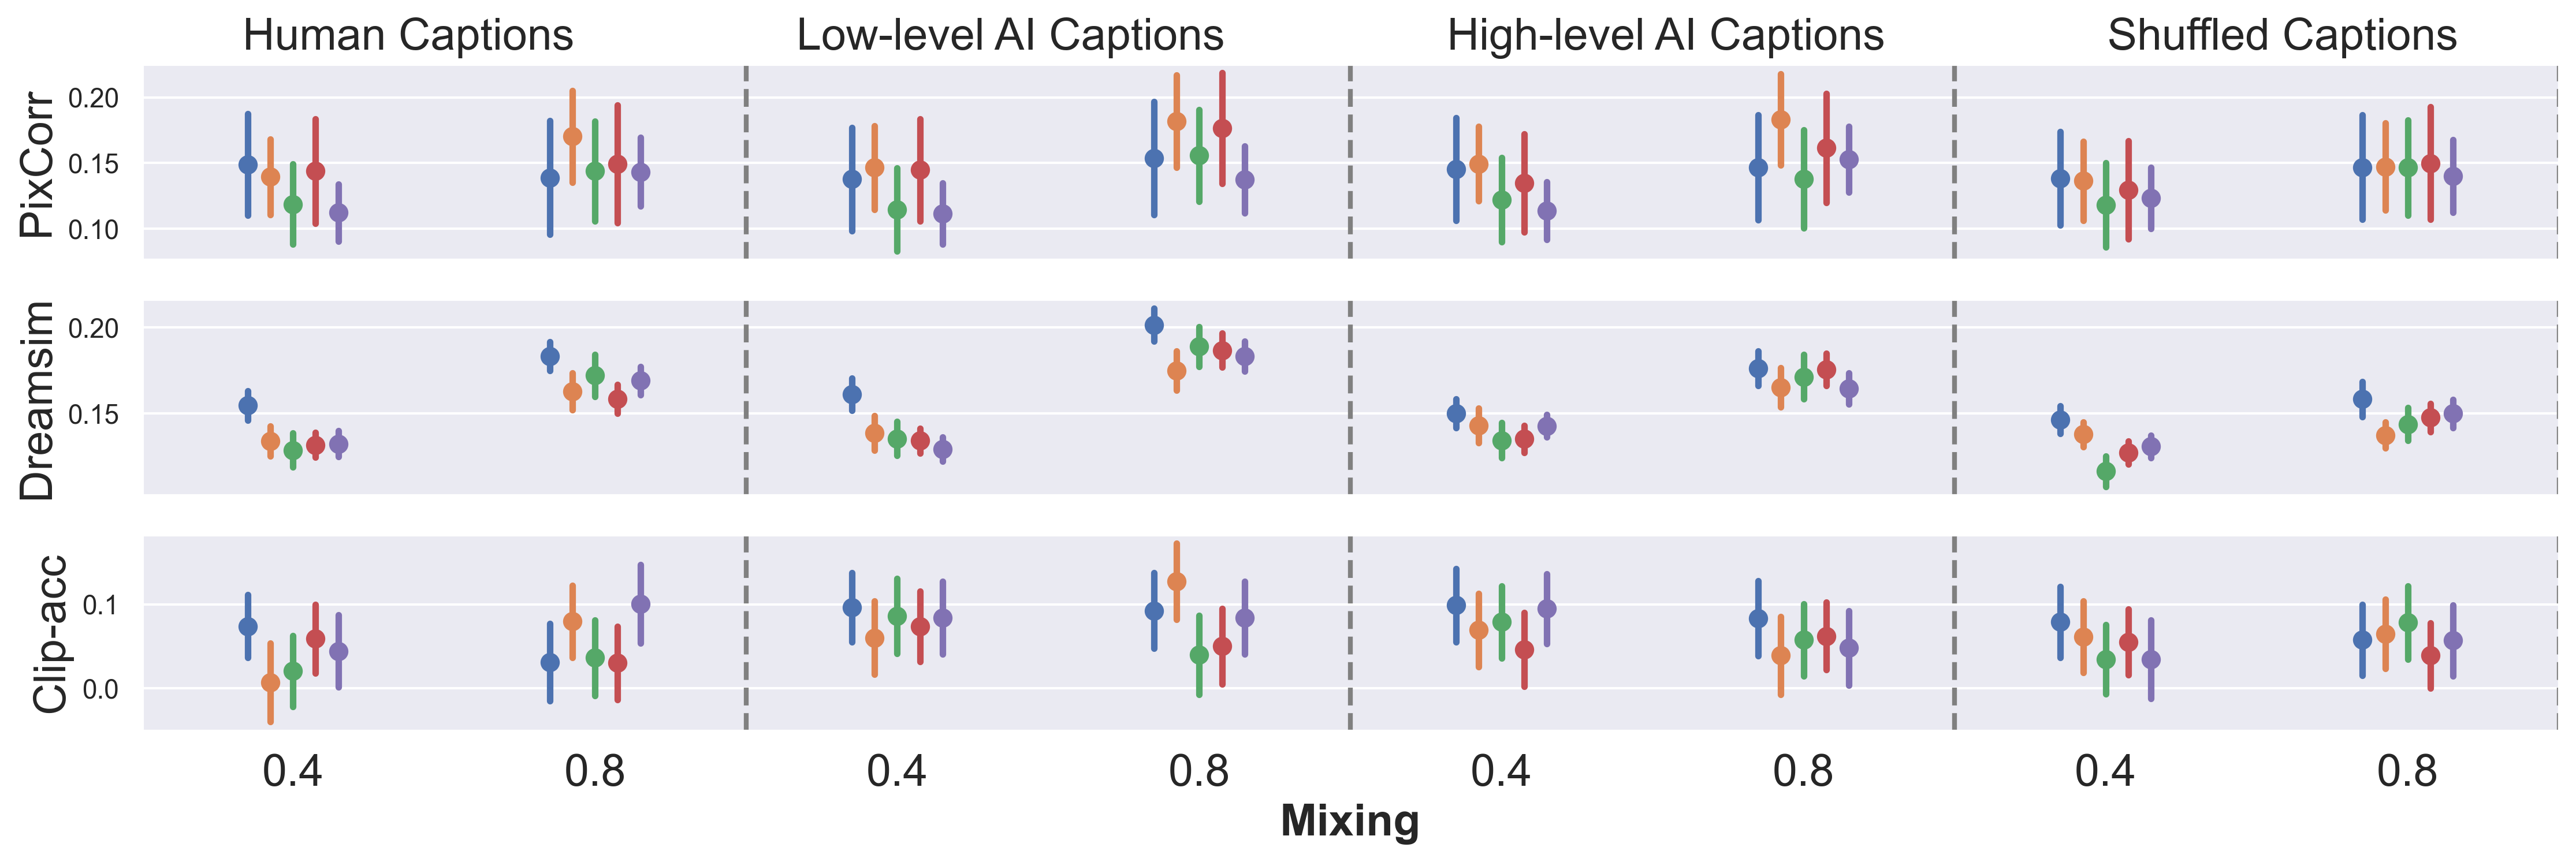
\includegraphics[width=1\textwidth]{plots/aicap_reconstruction_art_both_mixings.png}
    \caption{Reconstruction Artificial Images with different captions}\label{fig:aicap_reconstruction_art_both_mixings}
\end{figure}


% \begin{figure}[ht]
%     \centering
%     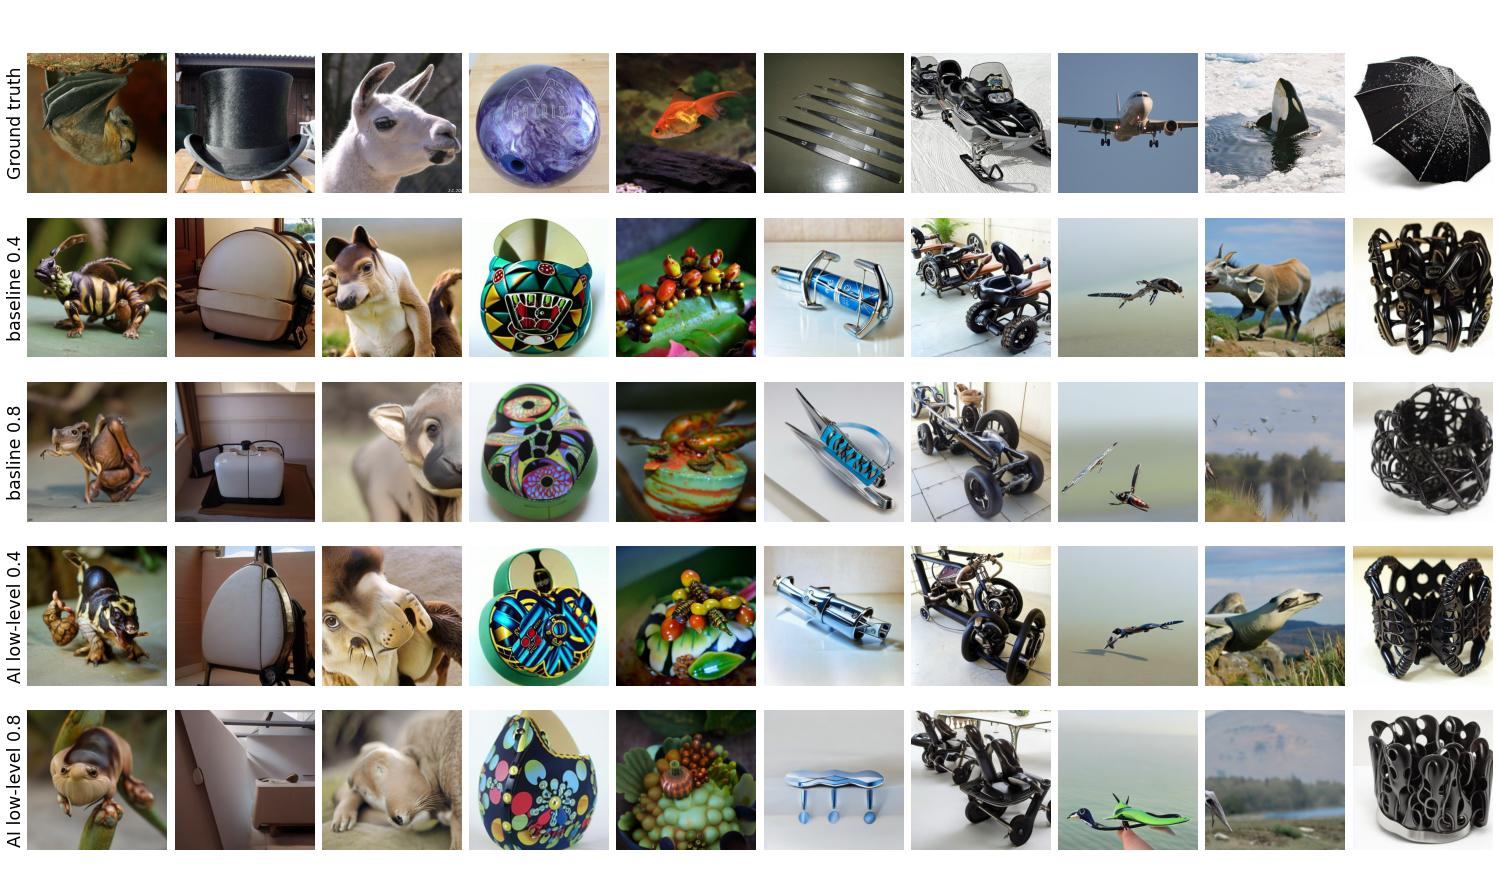
\includegraphics[width=0.6\textwidth]{plots/aicap_qual_test.JPEG}
%     \caption{AI-cap Reconstructions Natural Test Images}\label{fig:aicap_qual_test}
% \end{figure}

% \begin{figure}[ht]
%     \centering
%     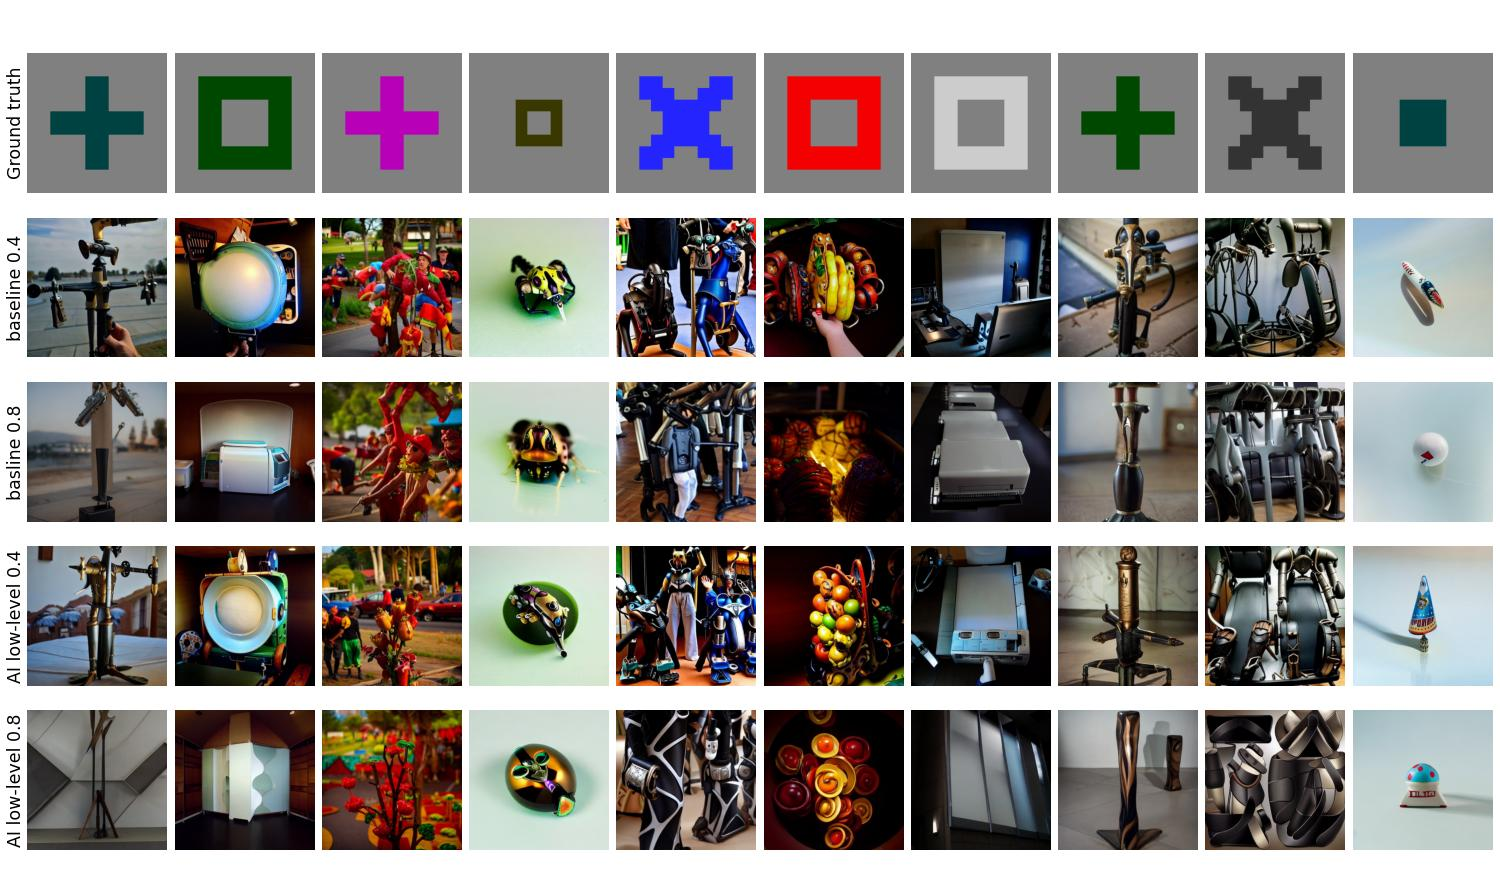
\includegraphics[width=0.6\textwidth]{plots/aicap_qual_art.JPEG}
%     \caption{AI-cap Reconstructions Artificial Shapes}\label{fig:aicap_qual_art}
% \end{figure}

\subsection{Discussion}

It could be shown that different types of captions, which refer to different features of the image, have a heterogeneous influence on the reconstruction performance. On the one hand, this confirmed the hypothesis that captions in the training data that refer to low-level features of the images can also ensure that the artificial shapes (which themselves do not carry much high-level information) can be better reconstructed. On the other hand, the reconstruction performance for natural images (which carry a lot of semantic meaning) was not reduced,  when the labels referred to the high-level information of the training images. PixelCorrelation did not prove to be a particularly good metric in this experiment, as it was able to detect an improvement in performance with increasing mixing in all cases (even with shuffled captions). The Dreamsim metric, on the other hand, best demonstrated the effect described above (low-level captions are good for artificial shapes and bad for natural test images). 

\begin{figure}[ht]
    \centering
    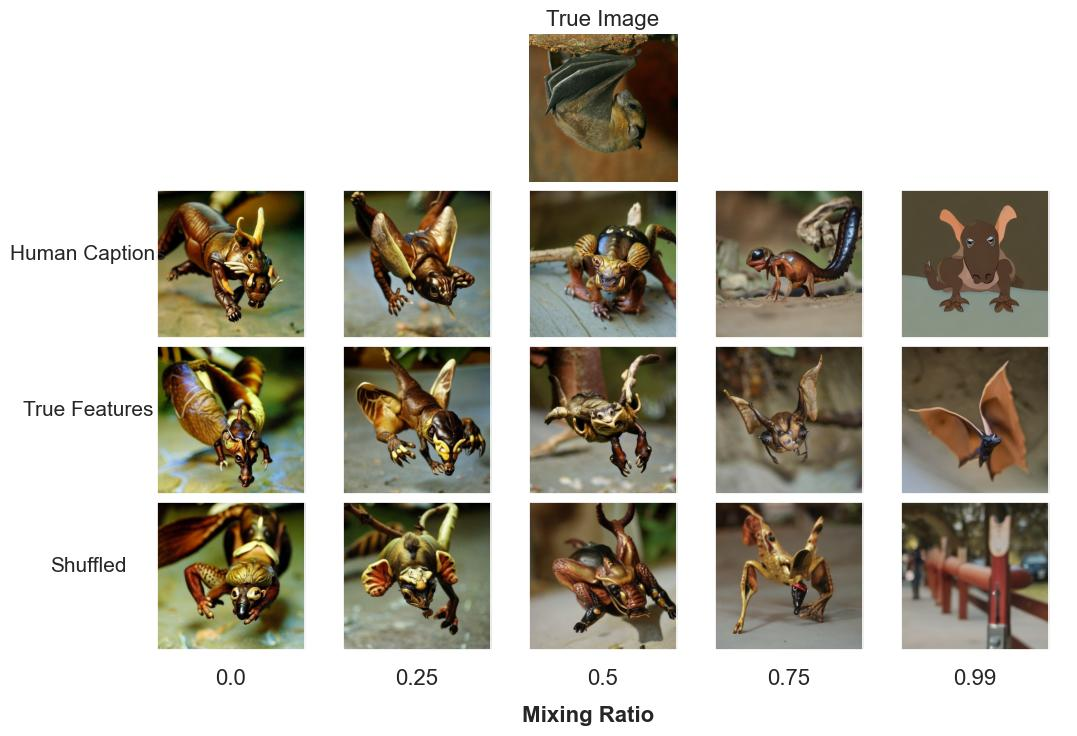
\includegraphics[width=0.8\textwidth]{plots/aicap_reconstruction_evolution_test_0.JPEG}
    \caption{AI-cap Reconstructions Artificial Shapes}\label{fig:aicap_reconstruction_evolution_test_0}
\end{figure}

For the natural test images and the artificial images, contrary effects were found as to whether increased mixing degrades (natural images) or improves (artificial shapes) the reconstruction performance. In order to identify the reason for this, a further analysis focused on the mixing parameter was conducted. Figure~\ref{fig:aicap_reconstruction_evolution_test_0} (and in the appendix in Figure~\ref{fig:aicap_reconstruction_evolution_art_0}) shows reconstructed images with increasing mixing ratios. In addition to the human and shuffled captions, the true features (i.e.\ the extracted clip text features of the images) are also used. It can be seen that as the mixing ratio increases, there is less detail in the image and the result becomes more blurred. This could be the explanation for the fact that the reconstruction performance (measured with dreamsim) for the natural test images decreases as the mixing ratio increases: because there is less detail in the reconstructed images, the naturalness (TODO quote) of the images decreases and they are less reminiscent of photorealistic images (the effect of the decreasing performance is shown quantitatively in Figure~\ref{fig:aicap_reconstruction_quant_evolution_test} in the appendix). This could also be the reason why the performance for the artificial images generally increases as the mixing ratio increases: because there is less (hallucinated) detail in the reconstructed images, the similarity to the low-detail artificial images increases (the increasing performance for the artificial images is shown in a quantitative manner Figure~\ref{fig:aicap_reconstruction_quant_evolution_art} in the appendix).



TODO: Überleitung dahin, dass mit den Captions der semantische Wert nicht besonders erhöht werden konnte, der Peak bei 0.4 erreicht ist, mit cliptext also nicht bedeutent die semantische Abbildung erhöht. Deshalb wollen wir an den anderen Teil vom Brain-difuser ran, clipvision. 